\chapter{User Manual}
\label{ch:usermanual}

	\section{Welcome}
	\label{sec:welcome}

		\begin{wrapfigure}{R}{0.25\textwidth}
			\vspace{-5em}
			\centering
			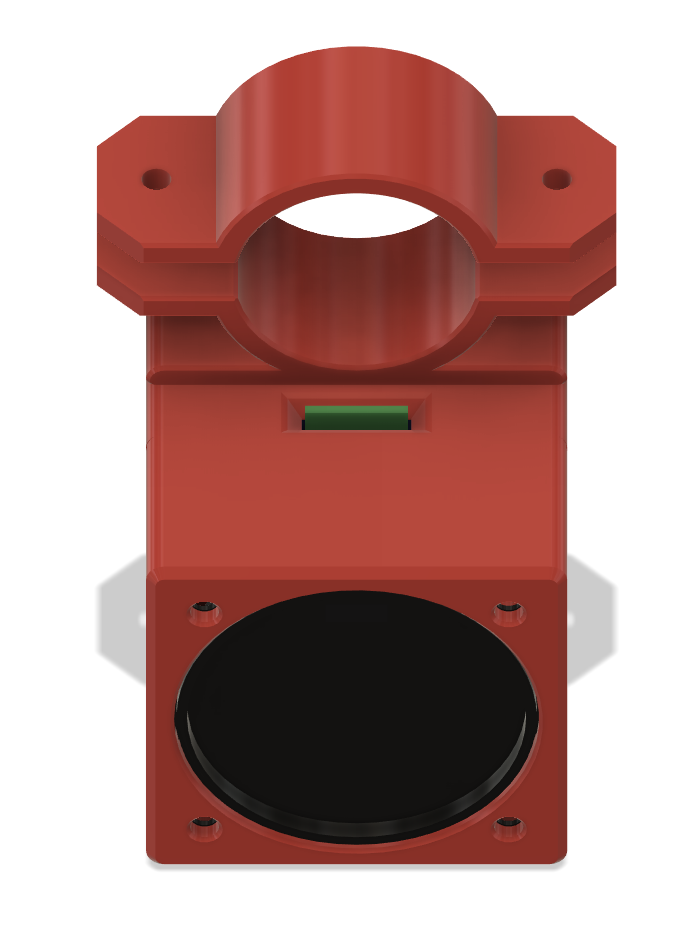
\includegraphics[width=0.25\textwidth]{graphics/final-cad.png}
		\end{wrapfigure}

		The Walking Aid Usage Prompt System is a medical aid consisting of a pair of hardware devices that allows patients suffering with dementia to be automatically reminded to use their walking aid when they begin walking without it. With stastically high rates of falling in dementia patients, the Walking Aid Usage Prompt System attempts to reduce these numbers. It aims to do this by offering a system that automatically detects when patients are walking without their walking aid and plays them a reminder to take their walking aid with them.

		\paragraph{Automatic Movement Detection}\mbox{}

		With the use of an accelerometer in each device, our systems can automatically detect when your patient is moving, and if they are moving without their walking aid.

		\paragraph{Remind the patient with the sound of a familiar voice}\mbox{}

		Utilising the SD card reader on the walking aid device, you can upload an MP3 file to be played to the patient when they begin walking without their walking aid. The connected speaker will give you the peace of mind that the patient will hear the reminder whenever it needs to be played.

		\begin{wrapfigure}{L}{0.25\textwidth}
			\vspace{-1em}
			\centering
			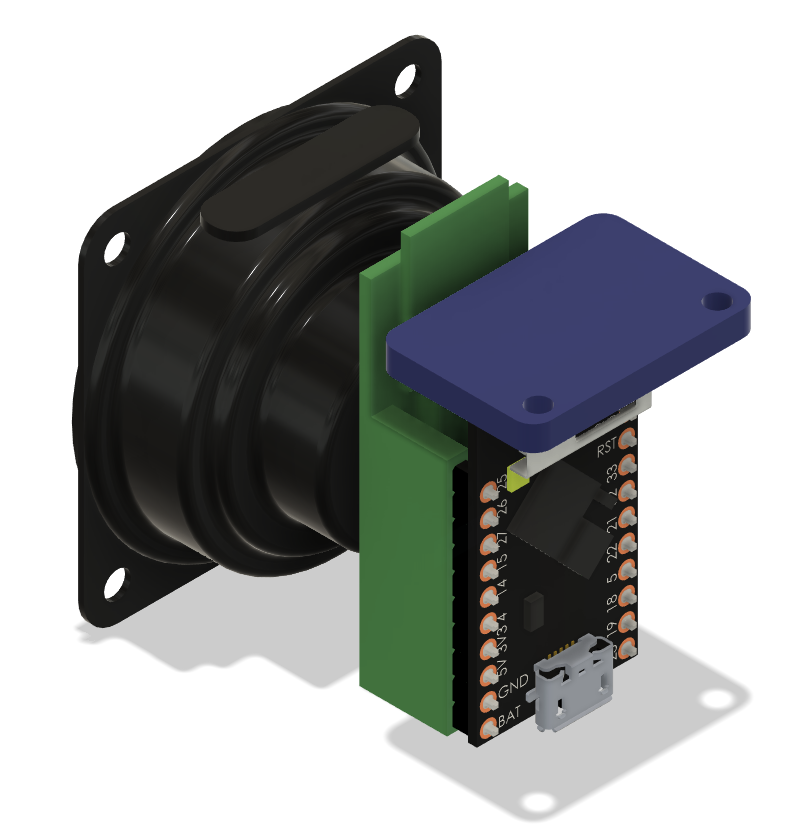
\includegraphics[width=0.25\textwidth]{graphics/hardware.png}
		\end{wrapfigure}

		\paragraph{Use a vibration reminder for patients who are hard of hearing}\mbox{}

		The inclusion of a communication protocol between our two devices will mean that the use of an audio reminder can be replaced, with the wearable device being asked to vibrate instead.

		\paragraph{Never use intrusive wearables again}\mbox{}

		Boasting a small form factor and the avoidance of distracting LEDs, our devices were developed with the comfort of the patient in mind. Utilising 18mm x 32mm TinyPICO development boards, our solution manages to keep device sizes to a minimum and can be worn on either the ankle or the wrist. 

		\paragraph{Next Steps:}\mbox{}

		\vspace{1em}
		Excited to get started?

		\textit{\hyperref[sec:quick_start_guide]{Click here for our Quick Start Guide} or head to section \ref{sec:quick_start_guide}}

		\vspace{1em}
		Want to learn more?

		\textit{\hyperref[sec:user_guide]{Click here for our more in depth User Guide} or head to section \ref{sec:user_guide}}

		\vspace{1em}
		Are you a developer?

		\textit{\hyperref[sec:developer_guide]{Click here to head to our developer guide} or head to section \ref{sec:developer_guide}}

	\newpage
	\section{Quick Start Guide}
	\label{sec:quick_start_guide}

		\subsection{Introduction}
		\label{subsec:quick_start_guide_introduction}

			The Walking Aid Usage Prompt system is a medical aid that allows patients to be automatically reminded to use their walking aid when they begin walking without it. The whole system comprises of two separate devices, one to be attached to the user's walking aid and the other to the ankle or wrist of the user. The wearable device is used to detect when the user has taken 5 steps within a 10 second period to signify that the user has began walking. Once this occurs, the wearable device communicates with the user's walking aid device to make a check to see if the walking aid is moving also. If the walking aid is moving, then great! There is no need to worry, the user is making use of their walking aid. However, should a user not be utilising their walking aid, then the walking aid can either play an audio reminder to the user, or it can communicate back to the wearable device to vibrate against the ankle or the wrist of the user. Both solutions are designed to remind the user to take their walking aid with them when walking in an attempt to reduce fall rates in dementia patients.

			The remainder of this quick start guide will explain the prerequisites to ensure that the system is fully functional, and a brief setup guide so that the user can get started.

		\subsection{Hardware Requirements}
		\label{subsec:quick_start_guide_hardware}

			\paragraph{To use the audio reminder system:}\mbox{}

			\begin{itemize}
				\item MicroSD Card >= 2MB Capacity.
				\item Windows/MacOS/Linux Computer System.
				\item A means to read/write to the SD card from the computer system. For example, a USB to MicroSD card reader.
				\item A microphone to record audio.
			\end{itemize}

			\paragraph{To use the vibration reminder system:}\mbox{}

			No hardware necessary, please advance to section \ref{subsec:quick_start_setup_guide}.

		\subsection{Software Requirements}
		\label{subsec:quick_start_guide_software}

			\paragraph{To use the audio reminder system:}\mbox{}

			\begin{itemize}
				\item Voice recording software such as Windows Voice Recorder or Audacity. (An alternative could be to record your voice message on a mobile device and transfer it to your computer system).
				\item File explorer software to copy the file to the SD card.
				\item MP3 audio file should be <= 2MB in size.
			\end{itemize}

			\paragraph{To use the vibration reminder system:}\mbox{}

			No software necessary, please advance to section \ref{subsec:quick_start_setup_guide}.

		\subsection{Setup Guide}
		\label{subsec:quick_start_setup_guide}

			\subsubsection{To use the audio reminder system}

				\paragraph{Getting your MicroSD card ready}\mbox{}

				To utilise the audio reminder system, you will need a MicroSD card with at least 2MB of storage capacity and an MP3 file that is less than 2MB in size. We recommend that the MP3 file include the voice recording of a relative, friend or carer that will remind the patient to use their walking aid. 

				\paragraph{Recording your reminder message}\mbox{}

				Using voice recording software and a microphone, record your voice message. Voice recording software can include the likes of:

				\begin{itemize}
					\item Windows Voice Recorder
					\item Audacity
					\item Mobile Device Voice Recording App such as Voice Recorder \& Audio Editor by TapMedia Ltd (iOS)
				\end{itemize}

				Should you need further assistance with recording your voice message, please see the full user guide \hyperref[sec:user_guide]{here} or head to section \ref{sec:user_guide}.

				\paragraph{Getting ready to transfer your file to the MicroSD card}\mbox{}

				Before getting started with the transferring of your MP3 file to the SD card, you will need to ensure that you have a means to read/write to the SD card. For example, a USB to MicroSD card reader that can connect to your computer system or mobile device, or computer system with a built in MicroSD card reader.

				It is imperative that your MicroSD card is using a FAT16/FAT32 file system to allow our devices to detect your audio file. Should your MicroSD card be using a different file system, please format your MicroSD card so that it is using a FAT16/FAT32 file system. WARNING! Formatting your MicroSD card will cause you to lose all of your data currently saved on it. Instructions for formatting your MicroSD card can be found below:

				\begin{itemize}
					\item \href{https://www.bu.edu/comtech/students/technical-guides/hardware/how-to-format-hard-drives/}{Format Instructions}
				\end{itemize}

				To transfer from your computer system to the MicroSD card, you will need to ensure that you file explorer software such as Windows Explorer or MacOS Finder ready to use.

				If you have recorded your voice message using a mobile device, you can either transfer your MP3 file to the computer system using a message system such as email or by connecting your mobile device to your computer system via USB. Another option is to connect your MicroSD card to your mobile device using one of the previously mentioned adapters to allow for file transfer.

				\paragraph{Transferring your MP3 file to the MicroSD card}\mbox{}

				Once you have access to writing to your MicroSD card, you are ready to transfer your MP3 file. Please follow the following steps to ensure that your MP3 file is transferred to the MicroSD card correctly to be fully functional with the Walking Aid Usage Prompt System:

				\begin{itemize}
					\item Open the file explorer software and locate your voice recorded MP3 file.
					\item Rename the file to 'reminder.mp3'.
					\item Through the file explorer software, locate your MicroSD card's storage location.
					\item Create a folder on the MicroSD card named 'reminder'.
					\item Copy and paste the 'reminder.mp3' file from your computer system/mobile device to the 'reminder' folder on the MicroSD card.
				\end{itemize}

				The process is now complete! You are ready to insert the MicroSD card into the walking aid device to begin using the system.

				\paragraph{Inserting you MicroSD card into the walking aid device}\mbox{}

				\begin{wrapfigure}{R}{0.25\textwidth}
					\vspace{-3.5em}
					\centering
					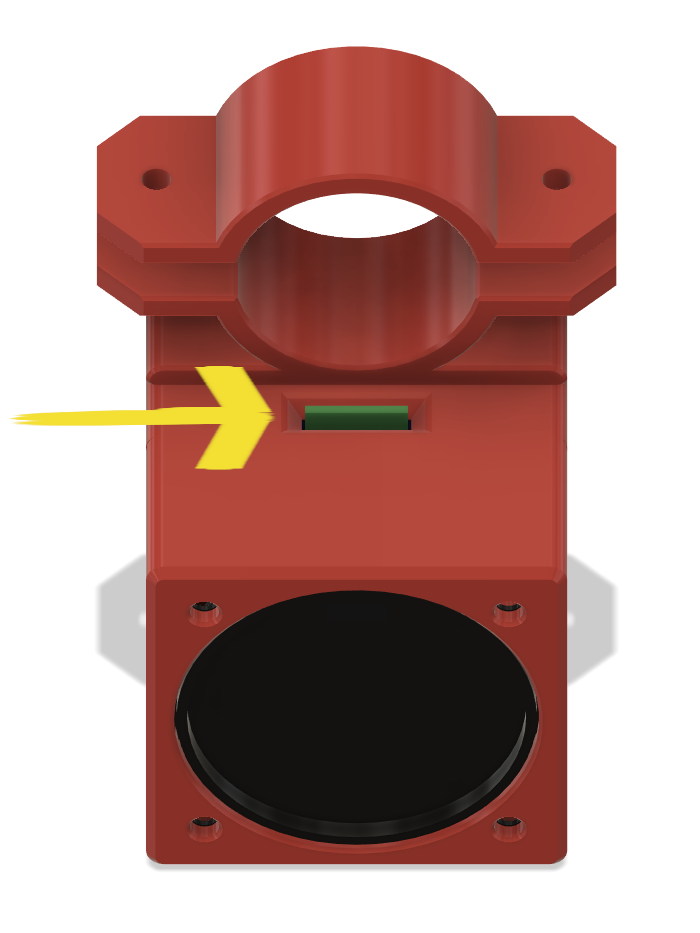
\includegraphics[width=0.25\textwidth]{graphics/sd_arrow.png}
				\end{wrapfigure}

				Once you have transferred your MP3 file to the MicroSD card, you will need to insert the MicroSD card into the walking aid device. You can insert the MicroSD card into the walking aid device by simply sliding the MicroSD card into the slot until you feel a click. The location of the MicroSD card slot can be seen in the image to the right. Once you have inserted the MicroSD card into the walking aid device, you are ready to power on your devices.

				\paragraph{Powering on your devices}\mbox{}

				Our current prototype lacks a battery powered solution, but one will be included in future work. For now, the devices require USB power, either from a battery bank or from a computer system. Once you have powered on your devices, you are ready to begin using the Walking Aid Usage Prompt System. To confirm that the device is functional, you should see the flash of a green LED for about one second.

				Should you notice any other LED light indicators, then please refer to the User Guide \hyperref[sec:user_guide]{here} or head to section \ref{sec:user_guide} for further troubleshooting instructions.

				\subsubsection{To use the vibration reminder system}

				As you are relying on the vibration reminder system, there is no need to utilise a MicroSD card, therefore you can skip to powering on the device. The design of our current prototype means that we will have setup the devices prior to you receiving them to ensure that they are functional for vibration reminders. Future work will be carried out to ensure that a button or switch system is implemented to allow the user to switch between vibration and audio reminders themselves.

				\paragraph{Powering on your devices}\mbox{}

				Our current prototype lacks a battery powered solution, but one will be included in future work. For now, the devices require USB power, either from a battery bank or from a computer system. Once you have powered on your devices, you are ready to begin using the Walking Aid Usage Prompt System. To confirm that the device is functional, you should see the flash of a green LED for about one second.

				Should you notice any other LED light indicators, then please refer to the User Guide \hyperref[sec:user_guide]{here} or head to section \ref{sec:user_guide} for further troubleshooting instructions.


	\section{User Guide}
	\label{sec:user_guide}

		\subsection{Troubleshooting LEDs}
		\label{subsec:troubleshooting_leds}

			\begin{tabular}{ m{0.1\linewidth} m{0.8\linewidth} } 

				\vspace{2em}
				
\includegraphics[width=0.5\linewidth]{graphics/green_circle.png}
				
				& You should see this LED for one second when you initally power on the device. This indicates that your device is functional. \\ 

				\vspace{2em}
				
\includegraphics[width=0.5\linewidth]{graphics/orange_circle.png}
				
				&  You are seeing this LED because the device in question is struggling to connect to the other device. Try powering them down, moving them closer together and restarting them. If you are still experiencing issues, please contact our support team here. \\ 

				\vspace{2em}
				
\includegraphics[width=0.5\linewidth]{graphics/red_circle.png}
				
				& This LED is being displayed as the initialisation of the communication protocol has failed. Please contact our support team here. \\
				 
			\end{tabular}

	\section{Developer Guide}
	\label{sec:developer_guide}

	% \section{Introduction}
	% \label{sec:usermanual_intro}

	% 	Intro on what the devices to, prerequisites, etc

		\todo{We probably need health disclaimers somewhere in our doc?}

	
	% \section{Hardware Guide}
	% \label{sec:usermanual_hardware}

	% 	Hardware stuff, powering on device, inserting sd card, assembly/dissasmbly guide? 

	% \section{Software Guide}
	% \label{sec:usermanual_software}

	% 	Software related things, setting device up with voice recording on sd card etc?


	% \section{Development Guide}
	% \label{sec:usermanual_development}

	% 	Code related guide
